\section{Introduction}\label{sec:intro}
%\textbf{Instructional Time:} 3 hours



\subsection{Prerequisites}\label{subsec:prerequisites}

This chapter assumes the reader has completed introductory courses in probability or statistics, and has completed the calculus series. We recommend ordinary differential equations but do not strictly require them. The Glossary (Section~\ref{sec:glossary}) at the end of the chapter collects unfamiliar terms and notation.


\subsection{The Problems with ODEs}\label{subsec:problems_with_odes}


Ordinary differential equations (ODEs) are a powerful modeling tool, but they have severe limitations. Some real-life phenomena evolve deterministically and continuously like a flowing river, and ODE models describe these very well. Others evolve \textit{stochastically} (which means \textit{randomly}), or discretely, or both. These phenomena behave more like a board game and, for these systems, ODE models require more thought to interpret.
Radioactive decay exemplifies the trouble, because it occurs per-atom and randomly. One atom unpredictably decays at a time, with random wait times between decay events.


\begin{example}\label{ex:radioactive_decay}
\textbf{Radioactive Decay.}
Rick has a radioactive isotope stored in Jerry's garage.
Let $\tau > 0$ be the half-life\index{half-life} measured in years.
Let $M_0$ be the mass at time $t=0$.
Let $M(t)$ denote the mass in grams of a radioactive isotope at time $t$ measured in years.
Assume the rate of change $\frac{dM}{dt}$ is proportional to $M(t)$. Then, for some proportionally constant $\mu > 0$, we have the following ODE.
\begin{equation}\label{eqn:radioactive_decay}
\frac{dM}{dt} = -\mu M.
\end{equation}
Equation~\ref{eqn:radioactive_decay} is the \textit{radioactive decay ODE}.
Since $M$ is in units of mass and $t$ is in units of time, $\frac{dM}{dt}$ has units of mass per time, so $\mu$ has units $(\text{time})^{-1}$.
We only have one equilibrium\index{equilibrium}, a point where all derivatives go to zero.
Namely, if $\frac{dM}{dt} = 0$, then $M = 0$.
Every real-valued trajectory with a positive initial condition $M_0 > 0$ has $\frac{dM}{dt} < 0$, and every real-valued trajectory with a negative initial condition $M_0 < 0$ has $\frac{dM}{dt} > 0$.
In this way, the equilibrium is globally stable\index{stable}.

The ODE is separable.
The solution trajectory $M(t)$ satisfies $\int \frac{dM}{M} = \int -\mu dt$.
Integrate both sides and collect the constants of integration to get $\ln\left|M\right| = -\mu t + c$.
Solve for $\left|M(t)\right| = e^{c-\mu t} = Ae^{-\mu t}$ for some constant $A=e^c$.
Substitute $t = 0$ to get $M(0) = M_0 = A$. Then the solution is $M(t) = M_0e^{-\mu t}$.
The constant of proportionality $\mu > 0$ is by assumption, but we are given the half-life $\tau$.
For a half-life $\tau$, $M(t)$ satisfies $M(t+\tau) = M(t)/2$ for all time $t$.
By direct substitution, we have $M(t+\tau) = M_0e^{-\mu(t+\tau)} = M_0 e^{-\mu \tau} e^{-\mu t}$.
Thus, $e^{-\mu \tau} = \frac{1}{2}$ so $\mu = \ln(2)/\tau$.
Substituting again yields $M(t) = M_0e^{-\frac{\ln(2)}{\tau} \cdot t} = M_0 2^{-t/\tau}$.

All solution trajectories $M_0 2^{-t/\tau}$ converge to $M = 0$ in the limit as $t \to \infty$, confirming the global stability of the equilibrium.
In Figure~\ref{fig:radioactive_decay}, we display a stream plot illustrating real-valued trajectories with different initial conditions.
Note that solutions to Equation~\ref{eqn:radioactive_decay} can be complex-valued.
Real-life matter has positive mass, so trajectories with complex or real negative $M(t)$ do not model real-life matter.
We shade this region red in Figure~\ref{fig:radioactive_decay}.
\end{example}

Even the strictly positive solutions $M(t) > 0$  for Example~\ref{ex:radioactive_decay} conflict with reality.
This ODE is \textit{homogeneous}\index{ODE!homogeneous}\index{homogeneous system of ODEs}\index{autonomous system|see{homogeneous system of ODEs}}\index{time-homogeneous system|see{homogeneous system of ODEs}}: its rate of change depends on the state alone, never explicitly on the clock $t$. We also call such a system \textit{autonomous} or \textit{time-homogeneous}. The Doob-Gillespie method developed in this chapter applies only to homogeneous ODEs.
Indeed, the model predicts the eventual occurrence of fractional masses of atoms, but the (integer) number of atoms determines the mass.
Thinking of half-life as ``time until exactly half the mass remains'' is a deterministic, continuous-state interpretation suggesting we can deterministically subdivide masses into halves forever.
Using this interpretation, the model in Equation~\ref{eqn:radioactive_decay} says ``after one half-life has elapsed, exactly half an atom is certain to remain.''
In contrast, real-life radioactive decay appears to be a stochastic (not deterministic) process governing a discrete (not continuous) mass quantized by number of atoms.
Fractional masses are not physical, but all the solutions in Figure~\ref{fig:radioactive_decay} spend most of their time in between integer values.

Because of these conflicts, interpreting the solutions of Equation~\ref{eqn:radioactive_decay} in the context of the original real-life problem requires additional intellectual framework.

\begin{example}\label{ex:logistic_growth}
\textbf{Logistic Growth Model.}
In 1857, Alexander Buchanan, overseer for Australian politician F. H. Dutton's Anlaby Estate in the Mid-North of South Australia, released a number of rabbits for hunting.
By 1867, the rabbit population in Australia was out of control.
Under optimal circumstances, rabbits take $4$ months to mature after birth and a female rabbit can give birth $6$ times a year to $6$ kits per litter.

Let $P(t)$ denote the population with per-capita rate of birth $r > 0$.
So, if we bring a mature male and mature female rabbit together at $t=0$ to breed, then $P(0)=P_0=2$ and after $2$ months, $P(2)=8$.
On the other hand, if a male and female are born at the same time at $t=0$ and breed when they are mature at $t=4$, then $P(0)=2$, and after $6$ months, $P(6)=8$.
For initial population $P_0 = P(0) > 0$, the classic population model is $\frac{dP}{dt} = rP$. Compare it to the radoiactive decay model. It has solutions $P(t) = P_0 e^{rt}$. These are unrealistic because they grow unboundedly.

Worse, the model requires high precision to parameterize. We say it is sensitive. For the rabbit population, we can estimate $r$ by using the two cases of rabbit breeding speed above. For the $P(2)=8$ case, $P(t) = 2 e^{rt}$ implies $P(2)=e^{2r}$. Solving for $r$ gives $r = \frac{1}{2}\ln(8) = \frac{3\ln(2)}{2} \approx 1.03972$. On the other hand, for the $P(6)=e^{6r}=8$ case, a similar argument suggests that $r = \frac{1}{6}\ln(8) = \frac{\ln(2)}{2} \approx 0.34657$. Both of these are estimates for a per-capita birth rate $r$,  a rabbit population will see average behavior somewhere between these two extremes. But, these are two very different values. A population with $r \approx 1.03972$ doubles about thrice as often as a population with $r \approx 0.34657$.

Instead of accepting the classic population model with unbounded solutions, we modify the ODE using an integer carrying capacity\index{carrying capacity} $0 < K \neq P_0$ and by assuming the \textit{effective} per-capita birth rate is $r(1-\frac{P}{K})\textup{ time}^{-1}$, providing the following.
\begin{equation}\label{eqn:logistic_growth}
\frac{dP}{dt} = r P\left(1-\frac{P}{K}\right)
\end{equation}
Equation~\ref{eqn:logistic_growth} is the \textit{logistic growth ODE}\index{logistic growth}.
The factor $(1 - P/K)$ is dimensionless ($P$ and $K$ share units) and acts as a correction to the per-capita birth rate $r$, reducing it linearly as $P$ approaches the carrying capacity $K$. In this way, we can account for the wide range of estimates of $r$ as dependent on sub-optimal rabbit-breeding conditions. Moreover, when $P/K \approx 0$, we have $\frac{dP}{dt} \approx rP$. From this point of view, effective per-capita birth rate can go at least as high as $1.03972$, and will drop as $P \to K$.
Equation~\ref{eqn:logistic_growth} is a separable ODE whose solutions satisfy $\int \frac{dP}{P(1-\frac{P}{K})} = \int r dt$.
Integrate both sides with partial fraction decomposition to get the solution.
\begin{equation}\label{eqn:logistic_solution}
P(t) = K\left(1 + \frac{K-P_0}{P_0}\,e^{-rt}\right)^{-1},
\end{equation}
Solutions to Equation~\ref{eqn:logistic_growth} can be complex-valued, but if they begin real, they stay real, and if they begin positive, they stay positive.  Certainly $P(0) = P_0$. Since $K > 0$, the signed coefficient $\frac{K-P_0}{P_0}$ has the same sign as $P_0$, compressing a sign convention into a convenient formula. Because $0 < r$, the term $e^{-rt} \to 0$ as $t \to \infty$, and hence $P(t) \to K$ for any $P_0 > 0$. Moreover, trajectories do not cross the lines $P = 0$ or $P = K$.
Every solution with $P_0 < 0$ blows up to $-\infty$ in finite forward time. To see why, write the solution as $P(t)=K/g(t)$ with $g(t)=1+A e^{-rt}$ and $A=\frac{K-P_0}{P_0}$.  Since $K>0$ and $P_0<0$, we have $K-P_0>0$, so $A<0$ with $|A|=\frac{K-P_0}{-P_0}=1+\frac{K}{-P_0} > 1$. Thus $g(0)=1+A=1-|A|<0$, while $g(t)\to 1>0$ as $t\to\infty$. Since $g$ is continuous and strictly increasing, $g$ has a unique root. Set $g(s) = 0$ and solve for $s=\frac{1}{r}\ln|A|>0$. On $[0,s)$ the denominator is negative and $g(t)\to 0^{-}$ as $t\to s^{-}$, so $P(t)=K/g(t)\to-\infty$. Hence the solution blows up at the finite time $s$.
That is to say, (i) every positive initial population, no matter how close to zero or how far it overshoots $K$, converges monotonically to $K$, (ii) every non-positive initial population escapes to $-\infty$ in finite time. The convergence of positive solutions stuck between $P = 0$ and $P = K$ is fastest where the absolute growth rate $rP\left(1-\frac{P}{K}\right)$ is largest, namely at $P=K/2$.

We call trajectories stuck between $P = 0$ and $P = K$ sigmoidal\index{sigmoidal curve} due to their $s$-shape. The point $P=K/2$, $f(P) = \frac{fK}{4}$ is exactly the inflection of one of these trajectories (about which the curve is horizontally symmetric). Solutions to this ODE appear in Figure~\ref{fig:logistic_growth}.


\begin{table}[htbp]
\centering
\begin{tabular}{llcl}
\hline
\textbf{Model} & \textbf{Event} & \textbf{Contribution to Rate of Change} & $\Delta$\textbf{State} \\
\hline \hline
Radioactive Decay & Decay & $\mu M$ & $-1$ atom \\ \hline
Logistic Growth & Birth & $rP$ & $+1$ organism \\
Logistic Growth & Death & $\frac{r}{K}P^2$ & $-1$ organism \\
\hline
\end{tabular}
\caption{Events, rates, and state changes for the radioactive decay and logistic growth models.}
\label{tab:ode_events}
\end{table}


\end{example}

The model in Equation~\ref{eqn:logistic_growth} suffers the same conceits as the radioactive decay model. Real-life masses are positive, so trajectories with complex or negative real $M(t)$ in the radioactive decay ODE have no physical interpretation. Similarly, real-life populations are positive, so trajectories with complex or negative real  $P(t)$ have no physical interpretations. Even the strictly positive solutions $P(t) > 0$ conflict with reality, predicting the eventual occurrence of a fractional population. This is a consequence of a deterministic, continuous-state interpretation of birth rate\index{birth rate} $r$ as related to ``time until the population exactly doubles.''

In the logistic growth model, events are individual birth and death events. Table~\ref{tab:ode_events} summarizes each event type, its rate, and its effect on the state for Example~\ref{ex:radioactive_decay} and Example~\ref{ex:logistic_growth}. Figure~\ref{fig:ode_examples} displays phase diagrams of Example \ref{ex:radioactive_decay} and Example \ref{ex:logistic_growth}.



\begin{figure}[htbp]
\centering
\begin{subfigure}[t]{0.48\textwidth}
\centering
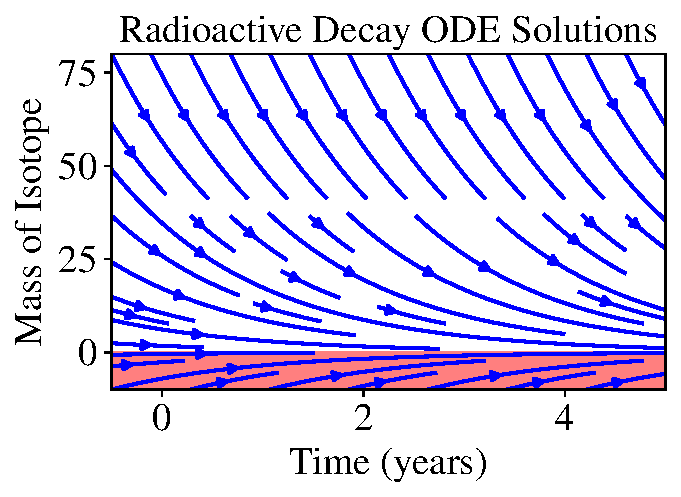
\includegraphics[width=\textwidth]{figures/radioactive_decay.pdf}
\caption{Radioactive decay ODE.}
\label{fig:radioactive_decay}
\end{subfigure}
\hfill
\begin{subfigure}[t]{0.48\textwidth}
\centering
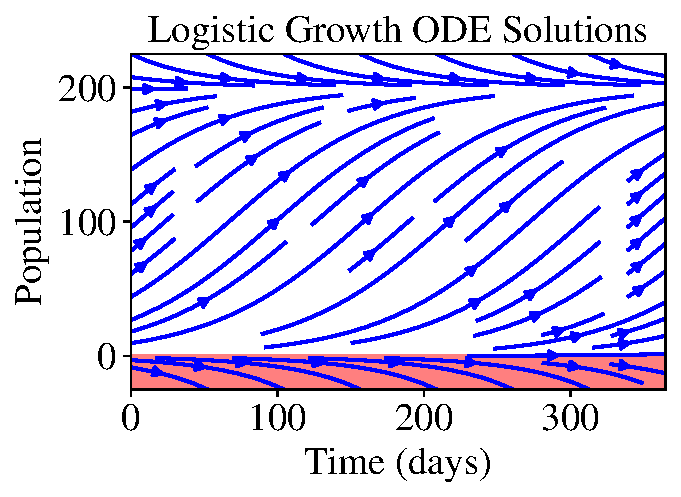
\includegraphics[width=\textwidth]{figures/logistic_growth.pdf}
\caption{Logistic growth ODE.}
\label{fig:logistic_growth}
\end{subfigure}
\caption{Phase diagrams for the two motivating homogeneous ODE models from Section~\ref{subsec:problems_with_odes}. The region below the $x$-axis (shaded red) has no physical meaning for matter isotopes. The companion Python repository on GitHub (see subsection \ref{subsec:companion_repo}) contains scripts that generate these images: \texttt{/stoch-ode/scripts/radioactive\_decay.py} and \texttt{/stoch-ode/scripts/logistic\_growth.py}. We draw both panels with \MakePhaseDiagram{} from \texttt{tools/plots/plot\_vector\_field.py} (Listing~\ref{lst:plots_vector_field}).}
\label{fig:ode_examples}
\end{figure}


Examples \ref{ex:radioactive_decay} and \ref{ex:logistic_growth} illustrate that interpreting the solutions to ODEs as describing a stochastic and discrete phenomenon requires additional intellectual framework.  System parameters and initial conditions uniquely determine solutions to suitably well-behaved ODEs, so we must account for the discrete state and stochasticity somewhere.


If the radioactive decay model is so problematic, why is it a canonical example of ODE modeling? Authors often conflate ODE solution trajectories with \textit{mean stochastic trajectories}.


\subsubsection{ODE trajectories are not mean stochastic trajectories}



Atoms are small in size and mass. A mole of atoms is a very large population ($6.023 \times 10^{23}$ atoms per mole) compared to human standards. So, the law of large numbers (LLN) and the Central Limit Theorem (CLT) both kick in when handling even relatively small masses by human standards. The LLN says behavior approaches the mean, and the CLT says behavior approaches a normal distribution, with a variance which gets tighter as sample size increases. So, the reasoning goes, a stochastic trajectory describing a large number of atoms behaves very close to the average. 

Should this not mean that the stochastic trajectories approach an ODE solution trajectory? Figure~\ref{fig:logistic_growth_mean_vs_ode} shows the logistic growth model over a short simulation window with a small sample. Over this window the dashed ODE solution and the solid stochastic mean trajectory track each other qualitatively.
Unfortunately (and contrary to popular belief) ODE solution trajectories do not generally match mean stochastic trajectories \cite{gillespie2009moment}.



\begin{figure}[htbp]
\centering
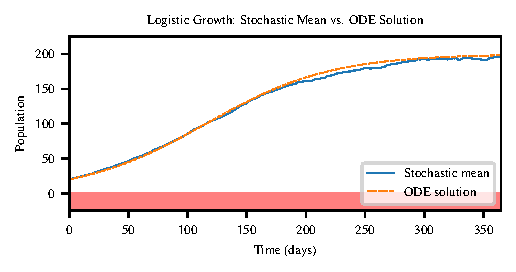
\includegraphics[width=\textwidth]{figures/logistic_growth_mean_vs_ode.pdf}
\caption{ODE solution (dashed) and Doob-Gillespie sample mean (solid), logistic growth model, $P(0) = K/2$. Short-time agreement masks qualitatively opposite long-run behavior. As usual, we shade non-physical regions red. We draw this with \PlotMeanVsOde{} from \texttt{tools/plots/plot\_mean\_vs\_ode.py} (Listing~\ref{lst:plots_mean_vs_ode}).}
\label{fig:logistic_growth_mean_vs_ode}
\end{figure}


To see why formally, note that Jensen's inequality\index{Jensen's inequality} states that, for a convex function $f$, the inequality $\mathbb{E}[f(P)] \geq f(\mathbb{E}[P])$ holds, with equality only when $f$ is affine or $P$ is almost surely constant. The death rate involves $P^2$, which is convex, so $\mathbb{E}[P^2] \geq (\mathbb{E}[P])^2$ in general. Therefore, the ODE governing $\mathbb{E}[P(t)]$ is (in general) not Equation~\ref{eqn:logistic_growth}. Modifying Equation~\ref{eqn:logistic_growth} to attain an ODE governing $\mathbb{E}[P(t)]$ requires adding higher-order terms estimated from higher-order statistical moments. We call this problem moment closure\index{moment closure} \cite{gillespie2009moment}, which lies beyond the scope of this text.

To see why more intuitively, note the long-run behaviors between exact ODE solution trajectories and stochastic realizations are qualitatively different. Consider the logistic growth model again. In the ODE, $P = K$ is a stable equilibrium: every trajectory that starts positive tends toward $P = K$ over time. The other equilibrium, $P = 0$, is unstable: a trajectory starting just above $0$ climbs toward $K$, and, as we showed above, a trajectory starting below $0$ escapes to $-\infty$ in finite time.

On the other hand, in the DG realization, stochastic trajectories do not stay at $P = K$ for long before stochastically jittering their way elsewhere. Trajectories are more likely to drift closer to $P=K$ than to drift away from $P=K$, but both are generally possible over small time intervals with strictly positive probability. Moreover, $P = 0$ is an absorbing state\index{absorbing state} for stochastic trajectories because the birth rate $rP$ and death rate $\frac{r}{K}P^2$ both vanish at $P = 0$. If the trajectory hits $0$, no further events are possible, and the population remains extinct permanently. 


Given any homogeneous ODE model whose stochastic realizations admit absorbing states, there is always a non-zero probability of a sequence of randomly sampled events which are unlucky, driving a stochastic trajectory into an absorbing state (if one exists). In fact, every step of the DG algorithm has such a probability. Generically, there is a minimum such probability $p$ for a fixed unit of simulated time $t$. We can then model which of the time intervals $[0, t)$, $[t, 2t)$, $\ldots$, $[kt, (k+1)t)$, $\ldots$ contains the extinction time as a geometric random variable. Each interval flips a coin with heads-up probability $p$, and extinction occurs in the first interval with a heads-up flip. The geometric random variable gives an upper bound on the time we expect to wait until we observe extinction. See Exercise \ref{ex:hw_bound_ext_time}.

If $P_{\texttt{ODE}}(t)$ is a solution to the ODE with a physical initial condition $P_{\texttt{ODE}}(0) > 0$, then $\underset{t \longrightarrow +\infty}{\lim} P_{\texttt{ODE}}(t) = K$. However, if $P_{\texttt{stoch}}(t)$ is a random variable describing stochastic trajectories with the same initial condition, then $\underset{t \longrightarrow +\infty}{\lim} \mathbb{E}[P_{\texttt{stoch}}(t)] = 0$. That is to say,
$$\underset{t \longrightarrow +\infty}{\lim} \mathbb{E}[P_{\texttt{stoch}}(t)] \neq \underset{t \longrightarrow +\infty}{\lim} P_{\texttt{ODE}}(t)$$ which shows that ODE solution trajectories are not mean stochastic trajectories. This argument is related to \textit{gambler's ruin}, the fact that a game with a negative expected value will eventually drive you broke, no matter your strategy. See Exercise \ref{ex:hw_gamblers_ruin}

The problem becomes more obvious when sample sizes get small and we can no longer fall back on the LLN and CLT, but the conceptual problem remains even with very large sample sizes. So, a non-trivial interpretation gap still confronts modelers after all the mathematics are said and done.







\textup{{\bf Questions for Reflection:}}
\begin{enumerate}
\item Examples~\ref{ex:radioactive_decay} and~\ref{ex:logistic_growth} are continuous-state, deterministic models, but they are modeling discrete-state, stochastic real-life systems. Provide examples of discrete-state, deterministic real-life systems?

\item Provide examples of continuous-state, stochastic real-life systems?

\item Do not fool yourself into thinking that discrete-state, deterministic processes are easy. For example, take any starting positive integer $x_0$ and, for each $i = 0, 1, 2, \ldots$, set the following.
\[x_{i+1} = \begin{cases}
\frac{x_i}{2};& x_i \textup{ is even} \\ 3x_i + 1;& x_i\textup{ is odd}
\end{cases}.\] Note that if any $x_i = 2^k$ for an integer $k > 0$, then $x_{i+k} = 1$. Investigate\footnote{Do not spend too much time on this question. Answering the question either way resolves a famously difficult, unsolved, addictive, and mysterious problem called the Collatz conjecture. The problem is sufficiently famous as to even appear in popular cinema, a dubious honor bestowed only upon the biggest wastes of time in mathematics.} whether every starting $x_0$ yields a sequence $(x_0, x_1, \ldots)$ which eventually terminates with some $x_i = 1$?
\end{enumerate}














\subsection{Structure of This Chapter}\label{subsec:structure}

The introductory chapter on the mathematical modeling process frames it as a \textit{modeling cycle} whose stages include \textit{getting a solution} and \textit{analysis and model assessment}. This chapter concentrates on those two stages. The Doob-Gillespie algorithm is our tool for getting a solution, and the parameter-sweep and sensitivity machinery supports analysis and model assessment.

\begin{itemize}
\item \textbf{Section~\ref{sec:resolving}: Resolving the Problem with Re-interpretation.} Re-interprets an ODE system as a discrete-state stochastic process. Identifies model events, derives the memoryless waiting-time distribution, and establishes the probability mass function (PMF) governing which event occurs next. The examples in this section already use integer-count units, so we require no rescaling.

\item \textbf{Section~\ref{sec:algorithm}: The Doob-Gillespie Algorithm in Detail.} Develops the full DG algorithm step by step, from the pre-processing rescaling (Step 0) through identifying events, sampling the waiting time, computing event rates, and choosing the next event.

\item \textbf{Section~\ref{sec:farming}: Doob-Gillespie Simulation Farming.} Builds DG implementations for the saline tank, logistic growth, Allee effect, and SIR models, and runs many simulations of each to estimate probabilities and summary statistics.

\item \textbf{Section~\ref{sec:visualizing_interpreting}: Visualizing and Interpreting Simulated Trajectories.} Plots individual trajectories as step graphs, aggregates many runs into heat maps, and introduces the sample statistics used to read stochastic output.

\item \textbf{Section~\ref{sec:parameter_sweep}: Parameter Space Exploration.} Introduces systematic exploration of a model across a grid of parameter values to survey qualitative behaviors and identify regions of interest.

\item \textbf{Section~\ref{sec:sensitivity_analysis}: Model Sensitivity Analysis.} Defines univariate elasticity, illustrates elasticity scoring on the logistic growth model, discusses bifurcations as qualitative regime changes, and cautions against elasticity comparisons that straddle a bifurcation point.

\item \textbf{Homework and Projects.} Homework problems reinforce the algorithmic steps. Projects are open-ended and intended as starting points for capstone or thesis investigations.

\item \textbf{Glossary.} Collects the probability and modeling terms used throughout the chapter. Consult it (Section~\ref{sec:glossary}) at the end of the chapter for any unfamiliar notation.
\end{itemize}


\subsection{Companion Python Repository on GitHub}\label{subsec:companion_repo}

 This chapter requires \texttt{Python 3.12} or later. We generate all simulations and figures in this chapter with programs and scripts written in \texttt{Python 3.12}.

To install \texttt{Python 3.12} in Windows or macOS, download and run the installer from \url{https://www.python.org/downloads/}. Otherwise, use your distribution's package manager (e.g., \texttt{sudo apt install python3} on Debian/Ubuntu). Verify the download by running \verb|python --version| in terminal. The output should begin with \texttt{Python 3.12} or higher. Our code targets \texttt{Python 3.12} or later. Readers on an older \texttt{Python} should upgrade before running the code. Our \texttt{Python} requires the \texttt{numpy} and \texttt{matplotlib} libraries. Install them via your \texttt{Python} distribution.

We host all \texttt{Python} code referenced in this chapter (scripts, simulation frameworks, and plotting utilities) at the \textbf{free} companion repository at \url{https://github.com/b-g-goodell/stoch-ode}.
\textit{Git} records the history of changes to a collection of
files. \textit{GitHub} hosts such histories and makes them publicly accessible. Students who intend to write and revise their own simulation code will find version control indispensable for keeping track of experiments and recovering from mistakes. The official tutorial at \url{https://git-scm.com/doc} is a
practical starting point. If you installed git, the following command downloads the repository into a new directory named \texttt{stoch-ode} automatically.
\begin{verbatim}
git clone https://github.com/b-g-goodell/stoch-ode
\end{verbatim}

Or, navigate to \url{https://github.com/b-g-goodell/stoch-ode}, see the repository directory structure plainly, and use \textit{Code $\to$ Download ZIP} to obtain the entire repository without Git.

The repository has the following directory structure. You can then run any script in the \texttt{scripts/} directory from within the repository directory with, for example,
\texttt{python scripts/logistic\_growth.py}. Readers who prefer interactive execution can open the scripts cell-by-cell in a \textit{Jupyter} notebook or \textit{Google Colab}.

\begin{table}[htbp]
\centering
\begin{tabular}{ll}
\hline
Directory & Contents \\
\hline
\texttt{scripts/}               & Top-level scripts for figures \\
\texttt{simulation\_frameworks/}& One framework per model \\
\texttt{tools/}                 & Plotting utilities and simulation core functions \\
\texttt{tests/}                 & Automated test suite, run with \texttt{pytest} \\
\hline
\end{tabular}
\caption{Top-level directories in the companion repository.}
\label{tab:repo_layout}
\end{table}




% Background Definitions moved to the end-of-chapter Glossary (sections/sec_11_glossary.tex).
